\documentclass [handout] {beamer}

\usepackage{graphicx, subfigure}
\usepackage{amsmath}


% \usepackage{beamerthemesplit} // Activate for custom appearance


\title{\color{blue}Metaknowledge Network Spring 2016}
\subtitle{\color{magenta}Introduction}
\author{ Nandana Sengupta}
\date{\color{blue}\today}

\begin{document}

\frame{\titlepage}

\frame{
\frametitle{About Me}
\begin{itemize}
\item<> Postdoc at Knowledge Lab
\vspace{2em}

\item<>Econometrics PhD

\vspace{2em}



\item<>{ \color{magenta}Research Focus:}
\begin{itemize}
\item<>Quantitative Methods
\item<>Public Policy Applications
\end{itemize}


\end{itemize}


}




\frame{
\frametitle{Projects at Knowledge Lab }
\begin{itemize}\small


\item<>{ \color{magenta}Focus:} Matrix Completion and Active Learning




\vspace{2em}

\item<>{ \color{magenta}Paper 1:  “A Matrix Factorization Approach to Multiple Imputation”}\\ (with Madeleine Udell, Nati Srebro, James Evans)
\item<>{ \color{magenta} Paper 2: “Active Learning applied to Online Social Surveys”}\\ (with Robert Nowak, Sumeet Kataria, James Evans)
\item<>{ \color{magenta} Paper 3: “Ratings, Rankings or Pairwise Comparisons?”} \\(with James Evans and Nati Srebro)


\end{itemize}


}



\frame{
\frametitle{Paper 1}
\begin{figure}[H]
\centering
\caption{Multiple Imputation Framework}
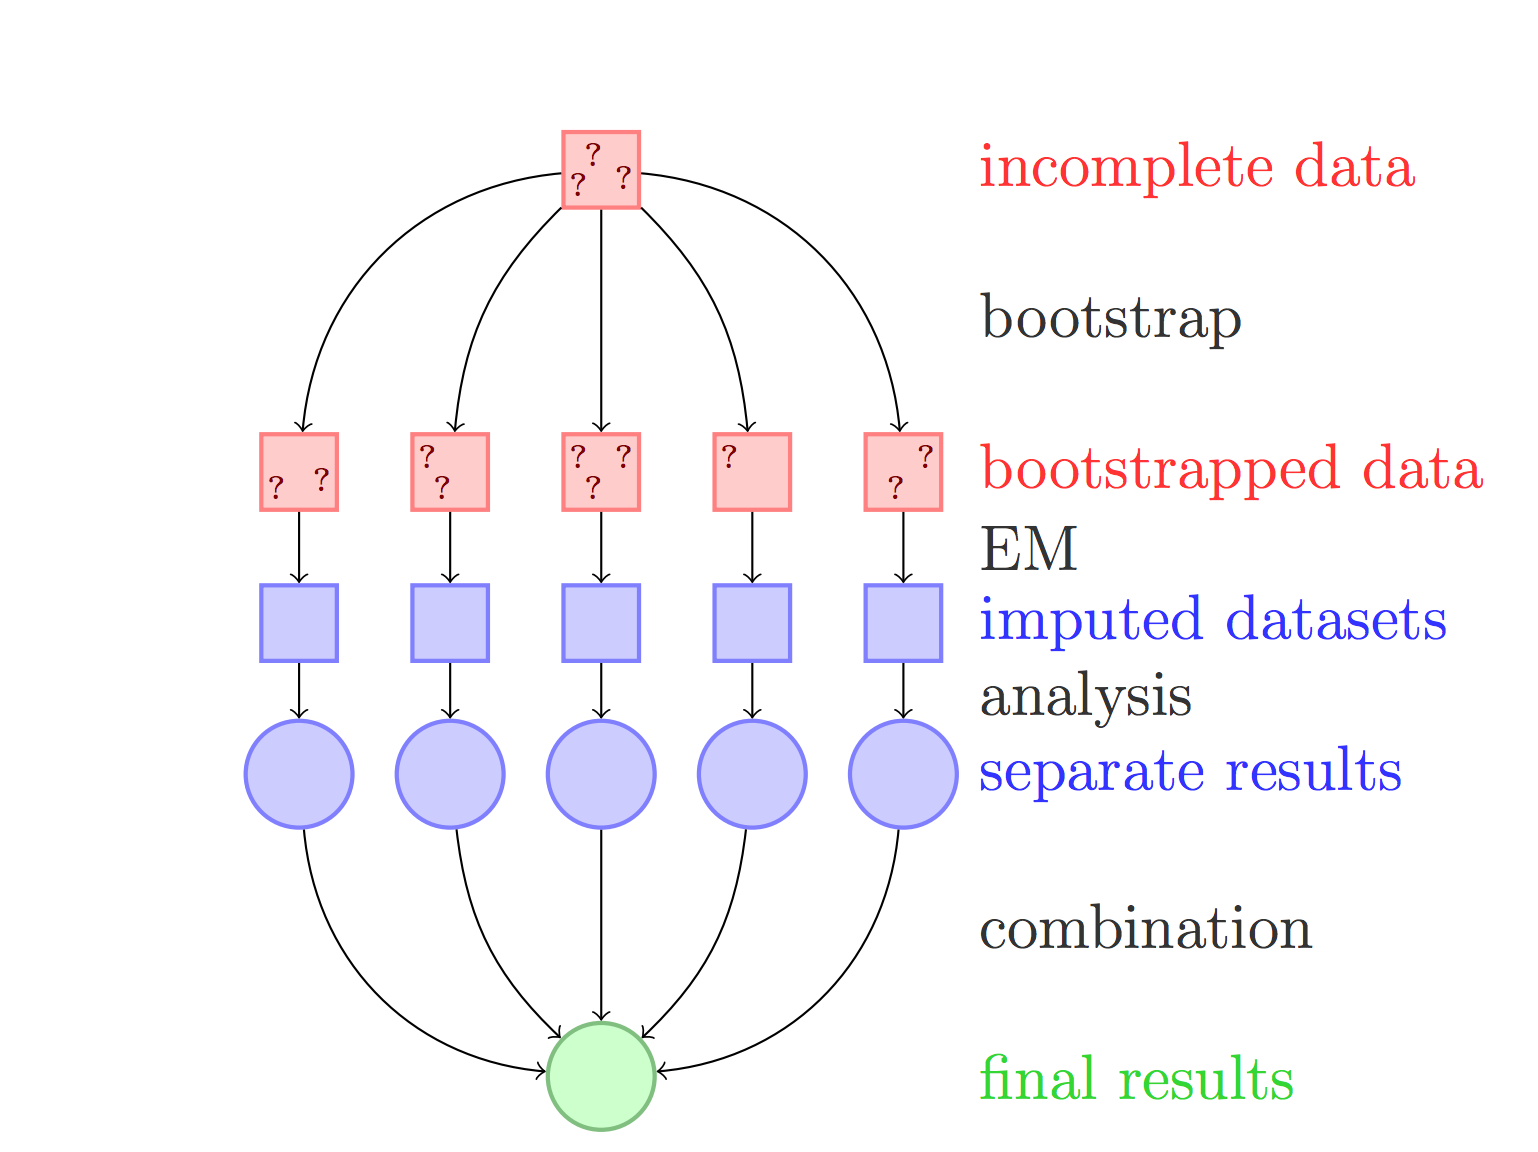
\includegraphics[width = 0.5\textwidth]{mult_imp}
\end{figure}
\begin{table}[H] \tiny
\centering
\begin{tabular}{|c|c|c|c|c|c|} 
  \hline
 & LowRank (S) & LowRank (NS) & Trace (FR) & Trace (LR) & MICE \\ 
  \hline
Scaled Loss/($10^3$) & 18.50 & 15.80 & 14.40 & 15.80 & 20.60 \\ 
  \%age reduction over MICE& 10.10   \%& 23.40  \% & 30.10  \% & 23.00  \% & -- \\ 
  \%age cols w/ lower loss & 73.50   \% & 84.60   \% & 87.20   \% & 84.60  \% & -- \\ 
   \hline
\end{tabular}
\end{table}





}



\frame{
\frametitle{Paper 2}


\includegraphics[width = 0.75\textwidth]{streetscore}
}



\frame{
\frametitle{Paper 2}

\textbf{Top 3 Predictors:} (office building, apartment building, hospital ) \\


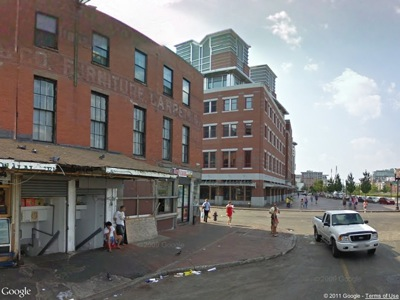
\includegraphics[width = 0.4\textwidth]{id_1_400_300.jpg}

\textbf{Top 3 Predictors:}(yard, residential neighborhood,  driveway) \\

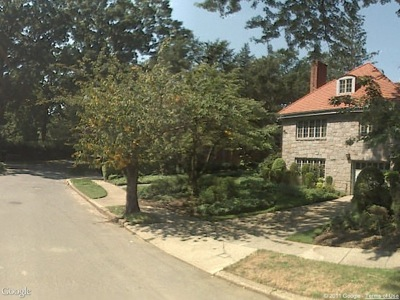
\includegraphics[width = 0.4\textwidth]{id_272_400_300.jpg}
}




\frame{
\frametitle{Paper 2}

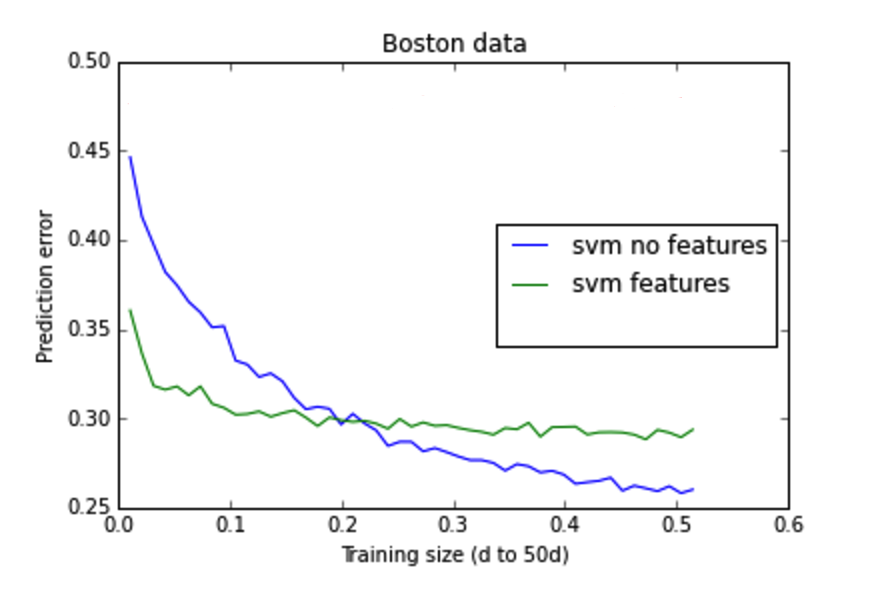
\includegraphics[width = 0.75\textwidth]{BostonData}
}





\frame{
\frametitle{Paper 3}

\includegraphics[width = 0.5\textwidth]{Rating}
}







\frame{
\frametitle{Paper 3}

\includegraphics[width = 0.35\textwidth]{Ranking}
}







\frame{
\frametitle{Paper 3}

\includegraphics[width = 0.5\textwidth]{Pairwise}
}







\frame{
\frametitle{Going Forward}
\begin{itemize}





\item<2-> Tensor Completion and Longitudnal Surveys
\item<3-> Public Policy Application of Caffe Feature Extraction and Neighborhood Safety 


\vspace{2em}

\item<4->Bandits in Public Policy Field Experiments 
\item<5->Machine Learning in Causal Inference 


\end{itemize}


}














\end{document}